\subsection{Support Vector Machines}
	Here, we present the theory for Support Vector Machines (SVMs) based on the lecture notes from Prof. Andrew Ng \cite{ng13}. SVMs are one of the most widely used and many argue among the best ``off-the-shelf'' supervised learning algorithms. This is mainly due to the sound theoretical framework, efficiency and good generalisation guarantees even for high-dimensional and linearly non-separable data.
	
\subsubsection{Notation}
	Having $m$ training examples, where
	\begin{itemize}

  		\item $\vec{x}^{(i)} \in \mathbb{R}^d$ is the $d$-dimensional $i$-th training example.
  		\item $y^{(i)} \in \left\{-1, 1 \right\}$ is the $i$-th training label.

	\end{itemize}
	we want to find the parameter $\vec{w} \in \mathbb{R}^d$ which describes the hyperplane $\vec{w}^T \vec{x} + b = 0$ that separates our two classes. Thus, we can define our classifier as $h_{\vec{w}, b}(\vec{x}) = g\left(\vec{w}^T \vec{x} + b \right)$, such that $g(z) = 1$ if $z \geq 0$ and $g(z) = -1$ otherwise. Note that this is a discriminative learning model as we are not modelling the joint probability of the data.
	
\subsubsection{Objectives}
	The essence of SVMs lies in finding the decision boundary (hyperplane) which maximises the gap between the closest training points to it. For the $i$-th training point $x^{(i)}$, we call the ``gap'', geometric margin $\gamma^{(i)}$, which is the distance to the decision hyperplane and can be found by considering a point $\vec{x}$ on it (note that $\vec{w}^T\vec{x} = -b$):
	\begin{align*}
		\gamma^{(i)} 	&= \left| \frac{\vec{w}^T}{\left\| \vec{w} \right\|} \left( \vec{x}^{(i)} - \vec{x} \right) \right| \\
					&= \frac{1}{\left\| \vec{w} \right\|} y^{(i)} \left( \vec{w}^T \vec{x}^{(i)} + b \right)
	\end{align*}
	However, we only consider the closest point $\vec{x}^{\left( i^\ast \right)} : i^\ast = \argmin_i{\gamma^{(i)}}$ with the geometric margin of $\gamma = \min_{i}{\gamma^{(i)}}$. Since scaling $\vec{w}$ and $b$ does not change the output of the classifier, nor the geometric margin $\gamma^{(i)}$, for convenience, we decide to scale $\vec{w}$ and $b$ such that $\left| \vec{w}^T \vec{x}^{(i^\ast)} + b \right| = y^{(i^\ast)} \left( \vec{w}^T \vec{x}^{(i^\ast)} + b \right) = 1$. Thus, maximising the geometric margin of the closest point becomes
	\begin{equation*}
	\begin{aligned}
		&\max_{\vec{w}, b} 		& & \frac{1}{\left\| \vec{w} \right\|} \\
		&\text{s.t.}				& & y^{(i)}(\vec{w}^T\vec{x}^{(i)} + b) \geq 1, &i=1,\dotsc,m.
	\end{aligned}
	\end{equation*}
	which is equivalent to
	\begin{equation}
	\begin{aligned}
		&\min_{\vec{w}, b} 	& & \frac{1}{2} \left\| \vec{w} \right\|^2 \\
		&\text{s.t.}				& & y^{(i)}(\vec{w}^T\vec{x}^{(i)} + b) \geq 1, &i=1,\dotsc,m.
	\end{aligned}
	\label{eqn:svm}
	\end{equation}
	The solution to the optimisation problem \eqref{eqn:svm}, which can be found using off-the-shelf Quadratic Programming (QP) packages, gives us the parameters required to do classification.

\begin{figure}[ht!]
	\centering
		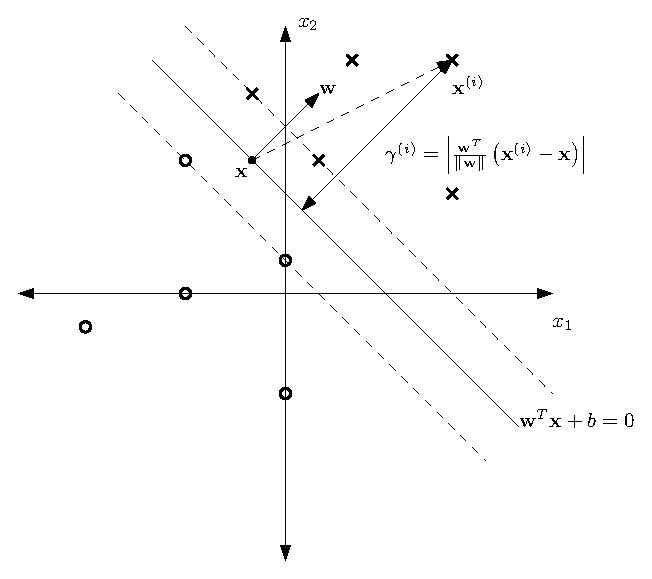
\includegraphics{drawings/svm.eps}
	\caption{Illustration of the optimal margin classifier.}
	\label{fig:svm}
\end{figure}

\subsubsection{Lagrange duality}
	While solving the optimisation problem \eqref{eqn:svm} using QP solves the problem, we move on to derive the dual form of the problem using the principle of Lagrange duality, which will help us to solve the problem using a more efficient algorithm. More importantly, it will also allow us to efficiently transform the data points to high-dimensional spaces using the ``kernel trick'', capturing the non-linear nature of the decision boundary without losing the generalisation guarantees. The Lagrangian of our primal minimisation problem \eqref{eqn:svm} (with parameters $\vec{\alpha} \in \mathbb{R}^m$) can be formed as
	\begin{equation}
		\mathcal{L}(\vec{w}, b, \vec{\alpha}) = \frac{1}{2} \left\| \vec{w} \right\|^2 - \sum_{i=1}^{m} \alpha_i \left[ y^{(i)}\left( \vec{w}^T \vec{x}^{(i)} + b \right) - 1 \right]
	\label{eqn:lagrangian}
	\end{equation}
	To find the dual form of the problem, $W(\vec{\alpha}) = \min_{\vec{w}, b} \mathcal{L}(\vec{w}, b, \vec{\alpha})$, we find the gradients of \eqref{eqn:lagrangian} with respect to $\vec{w}$ and $b$ and set them to zero to get
	\begin{align}
		\vec{w} 					& = \sum_{i = 1}^{m} \alpha_i y^{(i)} \vec{x}^{(i)} \label{eqn:dual1}\\
		\sum_{i = 1}^{m} \alpha_i y^{(i)}	& = 0 \label{eqn:dual2}
	\end{align}
	Substituting \eqref{eqn:dual1} and \eqref{eqn:dual2} back to \eqref{eqn:lagrangian} gives us the dual form, $W(\vec{\alpha})$
	\begin{equation}
		W(\vec{\alpha}) = \sum_{i = 1}^{m} \alpha_i - \frac{1}{2} \sum_{i, j = 1}^{m} y^{(i)} y^{(j)} \alpha_i \alpha_j \left\langle \vec{x}^{(i)}, \vec{x}^{(j)} \right\rangle
		\label{eqn:dualForm}
	\end{equation}
	Thus, under certain conditions which are in this case fulfilled (and omitted for clarity), our original optimisation problem \eqref{eqn:svm} becomes equivalent to the dual optimisation problem
	\begin{equation}
	\begin{aligned}
		& \max_{\vec\alpha}
		& & W(\vec{\alpha}) \\
		& \text{s.t.}
		& & \alpha_i \geq 0, & &  i = 1, \dotsc, m \\
		& & & \sum_{i = 1}^{m} \alpha_i y^{(i)} = 0, & &  i = 1, \dotsc, m
	\label{eqn:dualOpt}
	\end{aligned}
	\end{equation}
	This problem can be solved using a QP algorithm, however a more efficient Sequential Minimal Optimization (SMO) algorithm can be used. Once the optimal value  $\vec\alpha^\ast$ is obtained, we can find the corresponding parameters of the SVM $\vec w^\ast$ using \eqref{eqn:dual1} and $b^\ast$ using
	\begin{align}
		b^\ast 	& = - \frac{\max_{i: y^{(i)} = -1} {\vec w^*}^T \vec x ^{(i)} + \min_{i: y^{(i)} = 1} {\vec w^*}^T \vec x ^{(i)} }{2} \nonumber\\
				& = - \frac{\max_{i: y^{(i)} = -1} \sum_{j = 1}^{m} \alpha^\ast_i y^{(i)} \left\langle \vec{x}^{(i)}, \vec{x}^{(j)} \right\rangle + \min_{i: y^{(i)} = 1} \sum_{j = 1}^{m} \alpha^\ast_i y^{(i)} \left\langle \vec{x}^{(i)}, \vec{x}^{(j)} \right\rangle }{2} \label{eqn:bStar}
	\end{align}
	Thus the classification of a test point $\vec x$ can be done by evaluating the argument of $g({\vec w^\ast}^T \vec x + b^\ast)$
	\begin{equation}
		{\vec w^\ast}^T \vec x + b^\ast = \sum_{i = 1}^{m} \alpha_i^\ast y^{(i)} \left\langle \vec{x}^{(i)}, \vec{x} \right\rangle + b^\ast
		\label{eqn:svmClassifier}
	\end{equation}
	We note that due to certain conditions (Karush-Kuhn-Tucker conditions) the $\alpha^\ast_i$'s that are non-zero correspond to the $\vec x ^{(i)}$'s that lie on the margin. We call these points the Support Vectors (SVs). 

\subsubsection{Kernel trick}
	Note that according to \eqref{eqn:svmClassifier} (and \eqref{eqn:bStar}), we only need to evaluate the inner products of $\vec x$ and the support vectors in order to classify the point $\vec x$. This fact is used in the ``kernel trick'', in which a kernel function $K(\vec x, \vec z)$ is used as a proxy for the inner product $\langle \vec x, \vec z \rangle$. This effectively simulates transforming the data points to another, possibly unknown, space via a transformation function $\vec\phi (\cdot): \mathbb{R}^d \to \mathcal{Z}$ as long as there exists such $\mathcal{Z}$, i.e. there exists $\vec\phi (\cdot)$ such that $K(\vec x, \vec z) = \vec\phi (\vec x)^T \vec\phi (\vec z)$. It can be shown that a kernel $K(\cdot, \cdot)$ is valid if and only if it satisfies certain conditions called the Mercer's condtitions. This allows us to transform our input domain into much higher dimensional domains without actually doing so which turns out to improve the time complexity significantly.
	\begin{align}
		K_\text{poly}(\vec x, \vec z) & = \left( a \vec x^T \vec z  + c \right)^k \label{eqn:polyKernel} \\
		K_\text{rbf}(\vec x, \vec z) & = \exp{\left( - \frac{\left\| \vec x - \vec z \right\|^2}{2\sigma^2} \right)} \label{eqn:rbfKernel}
	\end{align}
	
	In our application, we are going to use the kernels above (\ref{eqn:polyKernel}, \ref{eqn:rbfKernel}). The first one, \eqref{eqn:polyKernel}, is the polynomial kernel which effectively transforms the input domain space into a feature space whose features are products all possible permmutations of the input features of degrees up to $k$. The second one, \eqref{eqn:rbfKernel}, is a radial basis kernel (RBF), whose corresponding transformation function transforms the input domain space to an infinite dimensional one. This kernel gives a large inner product to two points if they are close to each other.

\subsubsection{Soft margin SVMs}
	Soft margin SVMs are a slight modification of the original problem that allows small violations of the margin. The purpose is to guarantee that the algorithm doesn't fail because of the non-separability of the input data even after using the kernel trick. In practice, these two techniques are used simultaneously. It turns out that only minor changes arise and the SMO algorithm can still be used.
	
\subsubsection{Our problem}
	In our problem, we are going to use the \verb!SVM! package in \verb!MATLAB!\textsuperscript{\textregistered} in order to train our model and classify sleep apnoea. The package includes implementations of both QP and SMO algorithms, as well as various kernels, including the polynomial kernel and the RBF kernel. Recall that in our problem, we have the signal $\{ s_i \}_{i = 1}^T$ and the classifiers for every $K$ samples $\left\{ y_i \right\}_{i = 1}^{T/K}$, where $y_i \in \{0, 1\}$ classifies the time period represented by $\left\{ s_j \right\}_{j = (i - 1)K + 1}^{iK}$. When using SVMs, the input vectors and the classifiers become
	\begin{align*}
		\vec x^{(i)} 	& = [ s_{ (i - 1)K + 1}, \dotsc, s_{iK} ]^T \\
		y^{(i)} 	& = 
		\begin{cases}
			1	& \text{if } y_i  = 1 \\
			-1	& \text{otherwise.}
		\end{cases}
	\end{align*}